\documentclass[aspectratio=169,11pt]{beamer}
\usetheme{Madrid}
\usepackage[T1]{fontenc}
\usepackage{lmodern}
\usepackage{amsmath,amssymb}
\usepackage{booktabs,array}
\usepackage[table]{xcolor}
\usepackage{tikz}
\usetikzlibrary{arrows.meta,positioning,calc,shapes.geometric,decorations.pathreplacing}
\graphicspath{{../report/figures/}{./}}

\definecolor{iitblue}{RGB}{16,52,110}
\definecolor{accent}{RGB}{200,40,40}
\definecolor{good}{RGB}{20,120,60}
\definecolor{soft}{RGB}{235,240,248}
\setbeamercolor{structure}{fg=iitblue}
\setbeamercolor{palette primary}{bg=iitblue,fg=white}
\setbeamercolor{palette secondary}{bg=iitblue!85!black,fg=white}
\setbeamercolor{palette tertiary}{bg=iitblue!70!black,fg=white}
\setbeamercolor{frametitle}{bg=iitblue,fg=white}
\setbeamercolor{title}{bg=iitblue,fg=white}
\setbeamercolor{block title}{bg=iitblue,fg=white}
\setbeamercolor{block body}{bg=soft}
\setbeamercolor{block title alerted}{bg=accent,fg=white}
\setbeamercolor{block title example}{bg=good,fg=white}
\setbeamertemplate{navigation symbols}{}
\setbeamertemplate{itemize items}[circle]
\newcommand{\ours}{\rowcolor{good!15}}
\newcommand{\rstar}{r^{\ast}}

\title[Fronthaul Load Management for B5G]{Fronthaul Load Management for B5G Wireless Communications}
\subtitle{B.Tech. Project, Final Presentation}
\author[H. Choudhary, M. Yadav]{Harshvardhan Choudhary (230002027) \and Mayank Yadav (230002041)\\[4pt]
  {\small Guide: Dr. Sumit Gautam}}
\institute[IIT Indore]{Department of Electrical Engineering\\Indian Institute of Technology Indore}
\date{November 2026}
\titlegraphic{
\includegraphics[height=1.3cm]{IITI.png}}

\begin{document}

% ------------------------------------------------------------------ 1
\begin{frame}
\titlepage
\end{frame}

% ------------------------------------------------------------------ 2
\begin{frame}{Outline}
\begin{columns}[T]
\column{0.48\textwidth}
\begin{enumerate}
  \item Background: fronthaul, midhaul, backhaul
  \item Why the fronthaul is the bottleneck
  \item Problem statement
\end{enumerate}
\column{0.48\textwidth}
\begin{enumerate}\setcounter{enumi}{3}
  \item \textcolor{iitblue}{\textbf{Part A}}: make the data smaller and the DU faster
  \item \textcolor{accent}{\textbf{Part B}}: share one link well
  \item Part A $\times$ Part B, contributions, conclusion
\end{enumerate}
\end{columns}
\vspace{0.8cm}
\begin{block}{Guiding principle}
\centering Keep the mathematical structure of the problem, and learn only what is uncertain.
\end{block}
\end{frame}

% ------------------------------------------------------------------ 3
\section{Background}
\begin{frame}{How a phone reaches the Internet: fronthaul, midhaul, backhaul}
\centering
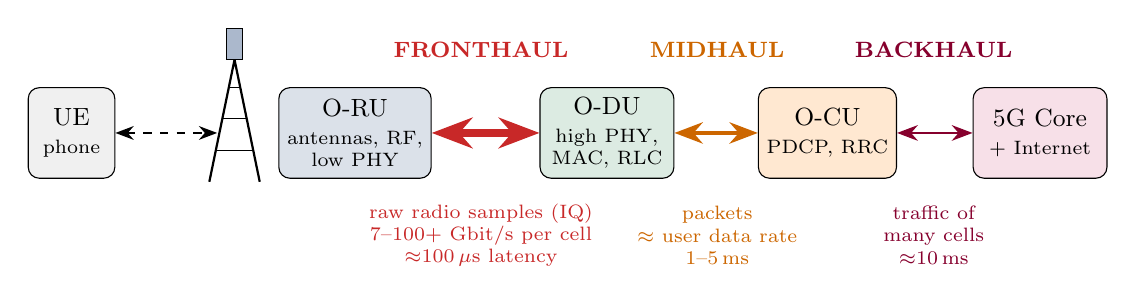
\begin{tikzpicture}[font=\small,>=Stealth,
  unit/.style={draw,rounded corners,align=center,minimum height=1.15cm,minimum width=1.7cm,inner sep=3pt},
  lbl/.style={font=\footnotesize\bfseries,align=center}]
  \node[unit,fill=gray!12,minimum width=1.1cm] (ue) at (0,0) {UE\\[-1pt]\scriptsize phone};
  \begin{scope}[shift={(1.75,-0.62)}]
    \draw[thick] (0,0) -- (0.32,1.55) -- (0.64,0);
    \draw (0.08,0.4) -- (0.56,0.4); \draw (0.16,0.8) -- (0.48,0.8); \draw (0.24,1.2) -- (0.40,1.2);
    \draw[fill=iitblue!35] (0.22,1.55) rectangle (0.42,1.95);
  \end{scope}
  \node[unit,fill=iitblue!15] (ru) at (3.6,0) {O-RU\\[-1pt]\scriptsize antennas, RF,\\[-3pt]\scriptsize low PHY};
  \node[unit,fill=good!15] (du) at (6.8,0) {O-DU\\[-1pt]\scriptsize high PHY,\\[-3pt]\scriptsize MAC, RLC};
  \node[unit,fill=orange!18] (cu) at (9.6,0) {O-CU\\[-1pt]\scriptsize PDCP, RRC};
  \node[unit,fill=purple!12] (core) at (12.3,0) {5G Core\\[-1pt]\scriptsize + Internet};
  \draw[<->,dashed,thick] (ue) -- (1.85,0);
  \draw[<->,line width=2.6pt,accent] (ru) -- (du);
  \draw[<->,line width=1.6pt,orange!80!black] (du) -- (cu);
  \draw[<->,line width=1.0pt,purple!70!black] (cu) -- (core);
  \node[lbl,text=accent] at (5.2,1.05) {FRONTHAUL};
  \node[lbl,text=orange!80!black] at (8.2,1.05) {MIDHAUL};
  \node[lbl,text=purple!70!black] at (10.95,1.05) {BACKHAUL};
  \node[font=\scriptsize,align=center,text=accent] at (5.2,-1.3) {raw radio samples (IQ)\\7--100+ Gbit/s per cell\\$\approx$100\,$\mu$s latency};
  \node[font=\scriptsize,align=center,text=orange!80!black] at (8.2,-1.3) {packets\\$\approx$ user data rate\\1--5\,ms};
  \node[font=\scriptsize,align=center,text=purple!70!black] at (10.95,-1.3) {traffic of\\many cells\\$\approx$10\,ms};
\end{tikzpicture}
\vspace{0.3cm}
\begin{itemize}\small
  \item \textbf{Fronthaul} (RU $\leftrightarrow$ DU): digitised radio waveform. Highest rate, tightest latency; a late packet is useless.
  \item \textbf{Midhaul} (DU $\leftrightarrow$ CU) and \textbf{backhaul} (CU $\leftrightarrow$ core): ordinary packet traffic, much lighter.
  \item Together they form the mobile transport network (``X-haul''). \textbf{This project is about the fronthaul.}
\end{itemize}
\end{frame}

% ------------------------------------------------------------------ 4
\begin{frame}{From D-RAN to Open RAN and the 7-2x split}
\centering
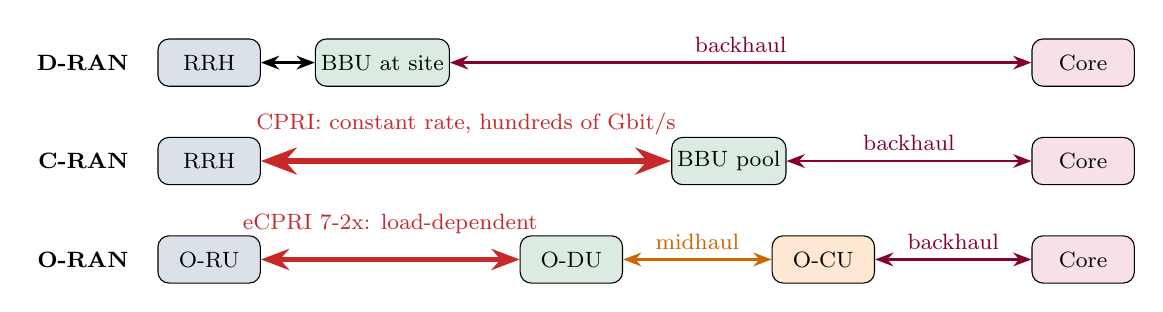
\begin{tikzpicture}[font=\footnotesize,>=Stealth,
  b/.style={draw,rounded corners,align=center,minimum height=0.6cm,minimum width=1.3cm,inner sep=2pt},
  row/.style={font=\footnotesize\bfseries,anchor=east}]
  \node[row] at (-0.5,0) {D-RAN};
  \node[b,fill=iitblue!15] (r1) at (0.4,0) {RRH};
  \node[b,fill=good!15] (b1) at (2.6,0) {BBU at site};
  \node[b,fill=purple!12] (c1) at (11.5,0) {Core};
  \draw[<->,thick] (r1) -- (b1);
  \draw[<->,thick,purple!70!black] (b1) -- node[above]{backhaul} (c1);
  \node[row] at (-0.5,-1.25) {C-RAN};
  \node[b,fill=iitblue!15] (r2) at (0.4,-1.25) {RRH};
  \node[b,fill=good!15] (b2) at (7.0,-1.25) {BBU pool};
  \node[b,fill=purple!12] (c2) at (11.5,-1.25) {Core};
  \draw[<->,line width=2.2pt,accent] (r2) -- node[above=5pt,text=accent]{CPRI: constant rate, hundreds of Gbit/s} (b2);
  \draw[<->,thick,purple!70!black] (b2) -- node[above]{backhaul} (c2);
  \node[row] at (-0.5,-2.5) {O-RAN};
  \node[b,fill=iitblue!15] (r3) at (0.4,-2.5) {O-RU};
  \node[b,fill=good!15] (d3) at (5.0,-2.5) {O-DU};
  \node[b,fill=orange!18] (u3) at (8.2,-2.5) {O-CU};
  \node[b,fill=purple!12] (c3) at (11.5,-2.5) {Core};
  \draw[<->,line width=1.6pt,accent] (r3) -- node[above=5pt,text=accent]{eCPRI 7-2x: load-dependent} (d3);
  \draw[<->,thick,orange!80!black] (d3) -- node[above]{midhaul} (u3);
  \draw[<->,thick,purple!70!black] (u3) -- node[above]{backhaul} (c3);
\end{tikzpicture}
\vspace{0.3cm}
\begin{itemize}\small
  \item \textbf{C-RAN} pools the baseband, but CPRI sends samples at a \emph{constant} rate $\propto$ bandwidth $\times$ antennas, even when the cell is idle.
  \item \textbf{O-RAN split 7-2x}: FFT stays in the O-RU; the fronthaul carries frequency-domain IQ \textbf{only for scheduled PRBs}, BFP compressed, over Ethernet.
  \item Fronthaul load now \textbf{follows the traffic}, so many cells can share one link.
\end{itemize}
\end{frame}

% ------------------------------------------------------------------ 5
\begin{frame}{Why the fronthaul is the bottleneck}
\begin{columns}[c]
\column{0.46\textwidth}
\resizebox{\linewidth}{!}{%
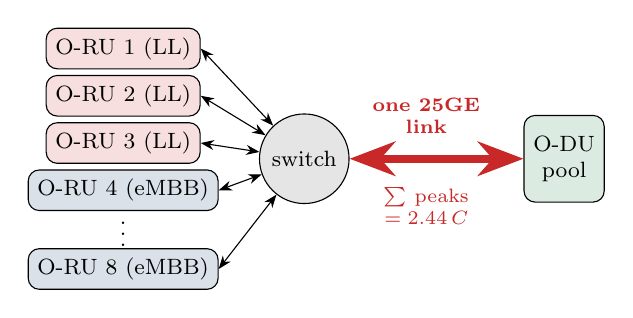
\begin{tikzpicture}[font=\footnotesize,>=Stealth,
   ru/.style={draw,fill=iitblue!15,rounded corners,minimum width=1.6cm,minimum height=0.5cm,align=center},
   ll/.style={draw,fill=accent!15,rounded corners,minimum width=1.6cm,minimum height=0.5cm,align=center}]
  \node[ll] (r1) at (0,2.4) {O-RU 1 (LL)};
  \node[ll] (r2) at (0,1.8) {O-RU 2 (LL)};
  \node[ll] (r3) at (0,1.2) {O-RU 3 (LL)};
  \node[ru] (r4) at (0,0.6) {O-RU 4 (eMBB)};
  \node at (0,0.15) {$\vdots$};
  \node[ru] (r8) at (0,-0.4) {O-RU 8 (eMBB)};
  \node[draw,fill=gray!20,circle,minimum size=0.9cm] (sw) at (2.3,1.0) {switch};
  \node[draw,fill=good!15,rounded corners,minimum height=1.1cm,align=center] (du) at (5.6,1.0) {O-DU\\pool};
  \foreach \r in {r1,r2,r3,r4,r8} \draw[<->] (\r.east) -- (sw);
  \draw[<->,line width=3pt,accent] (sw) -- (du);
  \node[text=accent,font=\scriptsize\bfseries,align=center] at (3.85,1.55) {one 25GE\\link};
  \node[text=accent,font=\scriptsize,align=center] at (3.85,0.4) {$\sum$ peaks\\$= 2.44\,C$};
\end{tikzpicture}}
\column{0.52\textwidth}
\small
\begin{alertblock}{1. Data are large, time is short}
BFP gives only $\approx$4$\times$. Every 0.5~ms slot the O-DU must invert a $K\times K$ matrix for all 273 PRBs: numpy + LAPACK needs \textbf{3.2~ms} for 16 users (6$\times$ the slot).
\end{alertblock}
\begin{alertblock}{2. The link is shared and smaller than the peak}
When bursts coincide, someone loses data. LL cells tolerate only 2~ms. Budgets must be set every 10~ms, \emph{before} the traffic is seen.
\end{alertblock}
\end{columns}
\end{frame}

% ------------------------------------------------------------------ 6
\begin{frame}{Problem statement and our two levers}
\centering
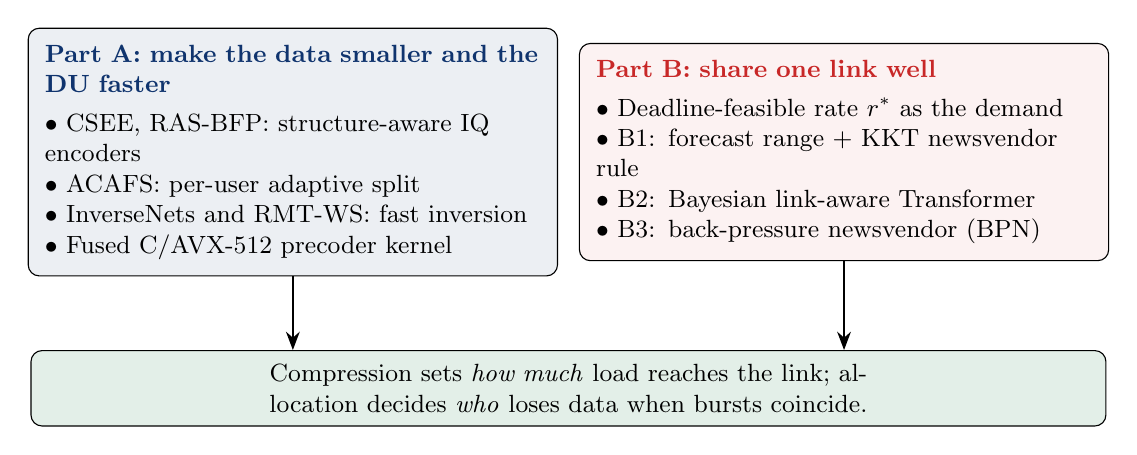
\begin{tikzpicture}[font=\small,>=Stealth,
   lever/.style={draw,rounded corners,align=left,text width=6.3cm,inner sep=6pt}]
  \node[lever,fill=iitblue!8] (A) at (0,0) {%
    \textbf{\textcolor{iitblue}{Part A: make the data smaller and the DU faster}}\\[3pt]
    $\bullet$ CSEE, RAS-BFP: structure-aware IQ encoders\\
    $\bullet$ ACAFS: per-user adaptive split\\
    $\bullet$ InverseNets and RMT-WS: fast inversion\\
    $\bullet$ Fused C/AVX-512 precoder kernel};
  \node[lever,fill=accent!6] (B) at (7.0,0) {%
    \textbf{\textcolor{accent}{Part B: share one link well}}\\[3pt]
    $\bullet$ Deadline-feasible rate $\rstar$ as the demand\\
    $\bullet$ B1: forecast range + KKT newsvendor rule\\
    $\bullet$ B2: Bayesian link-aware Transformer\\
    $\bullet$ B3: back-pressure newsvendor (BPN)};
  \node[draw,rounded corners,fill=good!12,text width=13.3cm,align=center,inner sep=5pt] (AB) at (3.5,-3.0) {%
    Compression sets \emph{how much} load reaches the link; allocation decides \emph{who} loses data when bursts coincide.};
  \draw[->,thick] (A.south) -- (A.south |- AB.north);
  \draw[->,thick] (B.south) -- (B.south |- AB.north);
\end{tikzpicture}
\end{frame}

% ------------------------------------------------------------------ 7
\section{Part A}
\begin{frame}{Part A: structure-aware IQ compression (CSEE and RAS-BFP)}
\begin{columns}[c]
\column{0.52\textwidth}
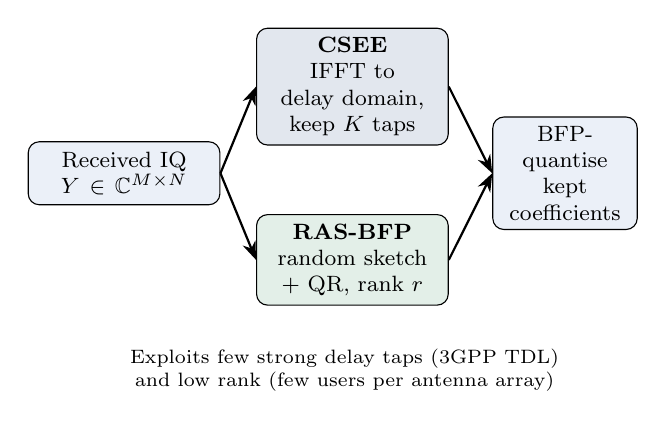
\begin{tikzpicture}[font=\footnotesize,>=Stealth,
   s/.style={draw,rounded corners,fill=soft,align=center,minimum height=0.8cm,text width=2.2cm}]
  \node[s] (y) at (0,0) {Received IQ\\$Y \in \mathbb{C}^{M\times N}$};
  \node[s,fill=iitblue!12] (c1) at (2.9,1.1) {\textbf{CSEE}\\IFFT to delay domain, keep $K$ taps};
  \node[s,fill=good!12] (c2) at (2.9,-1.1) {\textbf{RAS-BFP}\\random sketch + QR, rank $r$};
  \node[s,text width=1.6cm] (q) at (5.6,0) {BFP-quantise kept coefficients};
  \draw[->,thick] (y.east) -- (c1.west);
  \draw[->,thick] (y.east) -- (c2.west);
  \draw[->,thick] (c1.east) -- (q.west);
  \draw[->,thick] (c2.east) -- (q.west);
  \node[font=\scriptsize,align=center,text width=6.5cm] at (2.8,-2.5) {Exploits few strong delay taps (3GPP TDL)\\and low rank (few users per antenna array)};
\end{tikzpicture}
\column{0.46\textwidth}
\small
\begin{tabular}{lcc}
\toprule
Method & Ratio & Speed-up vs SVD \\
\midrule
O-RAN BFP & 3.9$\times$ & n/a \\
Truncated SVD & 16.2$\times$ & 1$\times$ \\
\ours \textbf{CSEE} & \textbf{12.7$\times$} & \textbf{4--6$\times$} \\
\ours \textbf{RAS-BFP} & \textbf{16.2$\times$} & \textbf{3--4$\times$} \\
\ours CSEE, $K{=}60$ & $\approx$\textbf{63$\times$} & n/a \\
\bottomrule
\end{tabular}

\vspace{0.2cm}
{\scriptsize at a target NMSE of about $-20$~dB}
\vspace{0.3cm}
\begin{itemize}
  \item Both encoders come with \textbf{provable NMSE bounds}.
  \item \textbf{3--4$\times$ more compression} than the O-RAN standard.
\end{itemize}
\end{columns}
\end{frame}

% ------------------------------------------------------------------ 8
\begin{frame}{Part A: ACAFS, a per-user adaptive functional split}
\begin{columns}[c]
\column{0.5\textwidth}
\begin{itemize}
  \item A fixed split is chosen at deployment for the worst case.
  \item ACAFS chooses the split \textbf{per user} from the channel rank that the encoder has already computed, so the choice costs nothing extra.
  \item Low rank: split 7-2x with compressed IQ is cheapest. High rank: moving more processing to the RU (split 7-1 or 6) sends fewer bits.
\end{itemize}
\column{0.46\textwidth}
\begin{exampleblock}{Result}
\centering
\Large \textbf{55--75\,\%}\\[2pt]
\normalsize bandwidth saving against a fixed Split~6 at high SNR
\end{exampleblock}
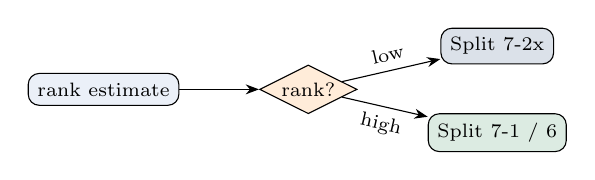
\begin{tikzpicture}[font=\scriptsize,>=Stealth]
  \node[draw,rounded corners,fill=soft] (r) at (0,0) {rank estimate};
  \node[draw,diamond,aspect=2,fill=orange!15,inner sep=1pt] (d) at (2.6,0) {rank?};
  \node[draw,rounded corners,fill=iitblue!15] (a) at (5.0,0.55) {Split 7-2x};
  \node[draw,rounded corners,fill=good!15] (b) at (5.0,-0.55) {Split 7-1 / 6};
  \draw[->] (r) -- (d); \draw[->] (d) -- node[above,sloped]{low} (a); \draw[->] (d) -- node[below,sloped]{high} (b);
\end{tikzpicture}
\end{columns}
\end{frame}

% ------------------------------------------------------------------ 9
\begin{frame}{Part A: fast matrix inversion for the precoder}
\small
RZF precoding needs $G^{-1}$, with $G = HH^H + \alpha I$, for every PRB in every 0.5~ms slot.
\begin{columns}[c]
\column{0.45\textwidth}
\centering
\begin{tabular}{lcc}
\toprule
Method ($n{=}100$) & Mean & p95 \\
\midrule
\ours \textbf{InverseNet-Ultra} & \textbf{0.47} & \textbf{0.57} \\
LAPACK \texttt{getri} & 0.57 & 1.13 \\
\ours InverseNet-NS & 0.97 & 1.06 \\
Newton--Schulz & 1.27 & 1.71 \\
Gauss--Jordan & 1.97 & 3.40 \\
LU (scipy) & 3.36 & 6.09 \\
SVD & 10.2 & 20.8 \\
QR & 20.3 & 64.5 \\
\bottomrule
\end{tabular}

{\scriptsize time in ms, CPU, one matrix at a time}
\column{0.52\textwidth}
\begin{itemize}
  \item 9-method benchmark; our learned \textbf{InverseNet-Ultra} has the \textbf{lowest mean latency} and \textbf{2$\times$ lower p95 than LAPACK}.
  \item It keeps the Newton--Schulz structure $X \leftarrow X(2I - GX)$ and learns only its coefficients.
  \item Lesson: \emph{learn the iteration, not the inverse}. This leads directly to RMT-WS.
\end{itemize}
\end{columns}
\end{frame}

% ------------------------------------------------------------------ 10
\begin{frame}{Part A: RMT-WS, random-matrix warm-start inversion}
\begin{columns}[c]
\column{0.5\textwidth}
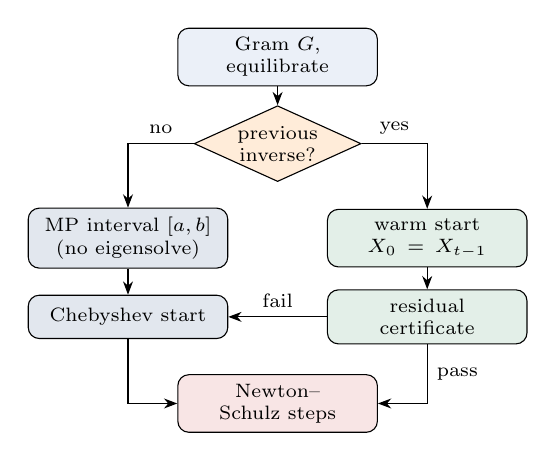
\begin{tikzpicture}[font=\scriptsize,>=Stealth,
  s/.style={draw,rounded corners,fill=soft,align=center,minimum height=0.55cm,text width=2.3cm},
  d/.style={draw,diamond,aspect=2.2,fill=orange!15,align=center,inner sep=0.5pt}]
  \node[s] (g) at (0,0) {Gram $G$, equilibrate};
  \node[d] (dec) at (0,-1.1) {previous\\inverse?};
  \node[s,fill=iitblue!12] (int) at (-1.9,-2.3) {MP interval $[a,b]$\\(no eigensolve)};
  \node[s,fill=iitblue!12] (ch) at (-1.9,-3.3) {Chebyshev start};
  \node[s,fill=good!12] (w) at (1.9,-2.3) {warm start\\$X_0 = X_{t-1}$};
  \node[s,fill=good!12] (c) at (1.9,-3.3) {residual\\certificate};
  \node[s,fill=accent!12] (ns) at (0,-4.4) {Newton--Schulz steps};
  \draw[->] (g) -- (dec);
  \draw[->] (dec.west) -| node[above,pos=0.25]{no} (int.north);
  \draw[->] (dec.east) -| node[above,pos=0.25]{yes} (w.north);
  \draw[->] (int) -- (ch); \draw[->] (w) -- (c);
  \draw[->] (c.west) -- node[above]{fail} (ch.east);
  \draw[->] (ch.south) |- (ns.west);
  \draw[->] (c.south) |- node[right,pos=0.25]{pass} (ns.east);
\end{tikzpicture}
\column{0.48\textwidth}
\small
\begin{itemize}
  \item Moment-matched \textbf{Marchenko--Pastur} interval: \textbf{100\,\% coverage}, also for correlated, near-far and LoS channels.
  \item \textbf{6 GEMMs} per inverse, where Neumann-type schemes need more than 10.
  \item Warm-start tracking: \textbf{2.25 steps per slot}, \textbf{0.006\,\%} sum-rate loss at walking speed.
  \item Closed-form \textbf{Doppler law} tells the O-DU in advance up to which speed warm start pays off.
\end{itemize}
\end{columns}
\end{frame}

% ------------------------------------------------------------------ 11
\begin{frame}{Part A: fused C/AVX-512 kernel on a real CPU}
\begin{columns}[c]
\column{0.5\textwidth}
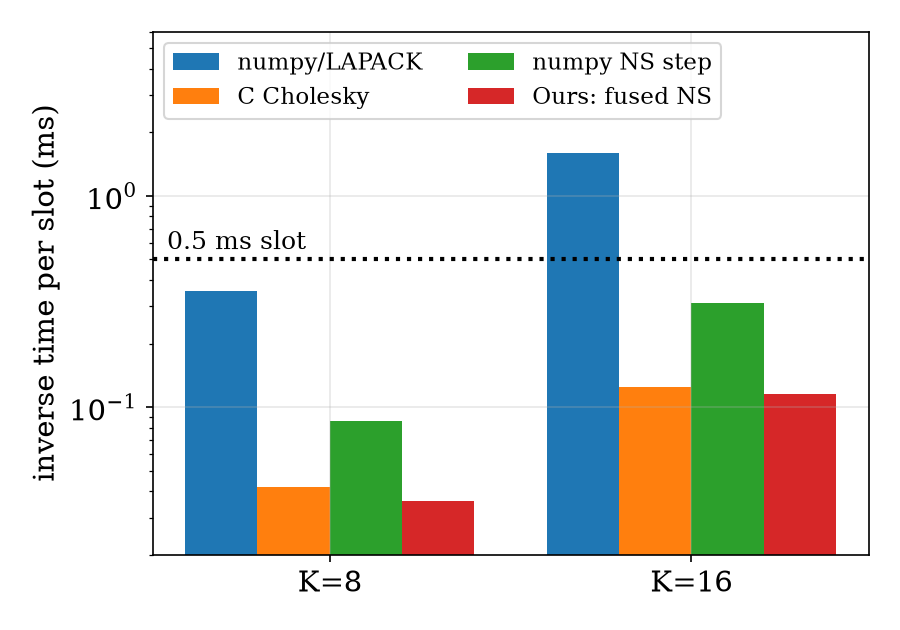
\includegraphics[width=\linewidth]{figures/inverse_kernel_slide.png}

{\scriptsize Inverse only: our fused Newton--Schulz step is the fastest inverse.}
\column{0.48\textwidth}
\small
\begin{tabular}{lcc}
\toprule
$K$, $M$ & numpy+LAPACK & \textbf{Ours} \\
\midrule
8, 64 & 1.08 ms & \textbf{0.070 ms} \\
\ours 16, 64 & 3.21 ms & \textbf{0.226 ms} \\
16, 128 & 4.71 ms & \textbf{0.41 ms} \\
\bottomrule
\end{tabular}

{\scriptsize whole precoder, 273 PRBs, 4 threads}
\vspace{0.2cm}
\begin{itemize}
  \item One fused pass per PRB: Gram, inverse, weights.
  \item \textbf{10--15$\times$ faster} than numpy + LAPACK; the whole precoder now \textbf{fits the 0.5~ms slot}.
  \item With RU-side precoding: \textbf{72\,\% less fronthaul} at 99.7\,\% of the exact sum-rate.
\end{itemize}
\end{columns}
\end{frame}

% ------------------------------------------------------------------ 12
\section{Part B}
\begin{frame}{Part B: system model and the deadline-feasible rate}
\small
\begin{itemize}
  \item 8 cells (3 LL with 2~ms deadline, priority 3; 5 eMBB with 10~ms, priority 1) share capacity $C$.
  \item Every $T = 10$~ms, on 1~ms-old telemetry, set budgets $r_i$ with $\sum_i r_i \le C$.
  \item Metric: priority-weighted violation ratio $\displaystyle V_w = \frac{\sum_i w_i\,\mathrm{violated}_i}{\sum_i w_i\,\mathrm{arrived}_i}$ (lower is better).
\end{itemize}
\begin{block}{Deadline-feasible rate: what a cell really needs}
\[
  \rstar(a, D) = \max_{s\le e} \frac{\sum_{t=s}^{e} a_t}{e - s + 1 + D},
  \qquad
  \text{need}_i = \underbrace{B_i}_{\text{clear backlog}} + \underbrace{\rstar_i}_{\text{future arrivals}}
\]
The smallest constant rate that delivers every bit before its deadline. Not the mean rate, not the peak.
\end{block}
\end{frame}

% ------------------------------------------------------------------ 13
\begin{frame}{B1: forecast a range, then split with the KKT newsvendor rule}
\begin{columns}[c]
\column{0.52\textwidth}
\small
Newsvendor view: reserve capacity under uncertain demand.
\[
  \max_{r}\ \sum_i w_i\,\mathbb{E}\big[\min(B_i + \rstar_i,\ r_i)\big]\ \ \text{s.t.}\ \sum_i r_i \le C
\]
\begin{block}{Closed-form KKT rule}
\[
  r_i(\lambda) = \mathrm{clip}\Big(B_i + F_i^{-1}\big(1 - \lambda/w_i\big),\,0,\,\mathrm{cap}_i\Big)
\]
one price $\lambda$ for the whole link, found by bisection
\end{block}
\begin{itemize}
  \item GBM quantile forecasts of $\rstar_i$; each cell gets its \emph{own} quantile level.
  \item Four proven properties; the KKT rule itself takes $<0.1$~ms.
\end{itemize}
\column{0.46\textwidth}
\scriptsize
\begin{tabular}{lccc}
\toprule
$V_w$ [\%], Family S & low & mod. & high \\
\midrule
Static equal share & 4.45 & 9.65 & 15.46 \\
Reactive proportional & 0.83 & 4.11 & 9.20 \\
MaxWeight & 0.90 & 4.85 & 11.54 \\
Deadline-aware reactive & 0.52 & 4.24 & 11.03 \\
Point forecast & 0.27 & 3.23 & 9.70 \\
\ours \textbf{Proposed (KKT)} & \textbf{0.15} & \textbf{2.15} & \textbf{8.00} \\
\bottomrule
\end{tabular}

\vspace{0.3cm}
\small
\begin{exampleblock}{Best of 12 controllers}
in every scenario of two traffic families; \textbf{11--43\,\%} fewer violations than the point forecast, \textbf{20/20 seeds}, $p<0.01$.
\end{exampleblock}
\end{columns}
\end{frame}

% ------------------------------------------------------------------ 14
\begin{frame}{B2: Bayesian link-aware Transformer forecaster (LCQT)}
\begin{columns}[c]
\column{0.5\textwidth}
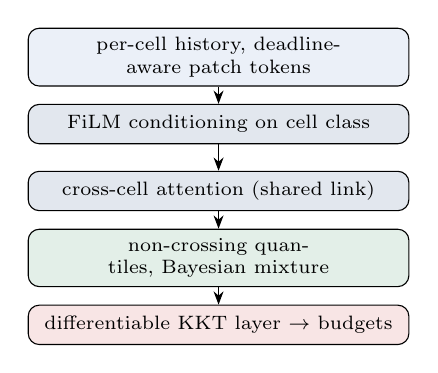
\begin{tikzpicture}[font=\scriptsize,>=Stealth,
  s/.style={draw,rounded corners,align=center,text width=4.6cm,minimum height=0.5cm}]
  \node[s,fill=soft] (a) at (0,0) {per-cell history, deadline-aware patch tokens};
  \node[s,fill=iitblue!12] (b) at (0,-0.85) {FiLM conditioning on cell class};
  \node[s,fill=iitblue!12] (c) at (0,-1.7) {cross-cell attention (shared link)};
  \node[s,fill=good!12] (d) at (0,-2.55) {non-crossing quantiles, Bayesian mixture};
  \node[s,fill=accent!12] (e) at (0,-3.4) {differentiable KKT layer $\rightarrow$ budgets};
  \draw[->] (a)--(b); \draw[->] (b)--(c); \draw[->] (c)--(d); \draw[->] (d)--(e);
\end{tikzpicture}
\column{0.48\textwidth}
\small
\begin{itemize}
  \item Learns calibrated joint quantiles of all cells together.
  \item Pinball loss \textbf{4.5\,\% lower} with the best calibration of all models.
\end{itemize}
\begin{center}
\begin{tabular}{lcc}
\toprule
Load & $V_w$ change & Seeds won \\
\midrule
low & $\mathbf{-20.8\,\%}$ & 20/20 \\
moderate & $\mathbf{-6.1\,\%}$ & 20/20 \\
high & $\mathbf{-1.4\,\%}$ & 20/20 \\
\bottomrule
\end{tabular}

{\scriptsize Bayesian LCQT + KKT vs.\ GBM + KKT (B1)}
\end{center}
\end{columns}
\end{frame}

% ------------------------------------------------------------------ 15
\begin{frame}{B3: the back-pressure newsvendor (BPN)}
\begin{columns}[c]
\column{0.5\textwidth}
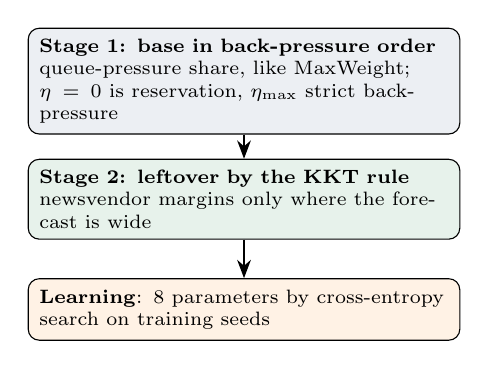
\begin{tikzpicture}[font=\scriptsize,>=Stealth,
   s/.style={draw,rounded corners,align=left,text width=5.2cm,inner sep=4pt}]
  \node[s,fill=iitblue!8] (st1) at (0,0) {\textbf{Stage 1: base in back-pressure order}\\
    queue-pressure share, like MaxWeight;\\$\eta=0$ is reservation, $\eta_{\max}$ strict back-pressure};
  \node[s,fill=good!10] (st2) at (0,-1.5) {\textbf{Stage 2: leftover by the KKT rule}\\
    newsvendor margins only where the forecast is wide};
  \node[s,fill=orange!10] (cem) at (0,-2.9) {\textbf{Learning}: 8 parameters by cross-entropy search on training seeds};
  \draw[->,thick] (st1) -- (st2); \draw[->,thick] (st2) -- (cem);
\end{tikzpicture}
\vspace{0.1cm}

\small Contains both strongest baselines \emph{exactly} (predictive MaxWeight, CEM policy).
\column{0.48\textwidth}
\scriptsize
\begin{tabular}{lccc}
\toprule
$V_w$ [\%], Family S & low & mod. & high \\
\midrule
KKT rule (B1) & 0.15 & 2.15 & 8.00 \\
Pred.\ MaxWeight & 0.16 & 1.66 & 5.98 \\
CEM policy & 0.13 & 1.73 & 6.58 \\
\ours \textbf{BPN} & \textbf{0.10} & \textbf{1.21} & \textbf{5.23} \\
\ours \textbf{BPN + Bayesian LCQT} & \textbf{0.08} & \textbf{1.11} & \textbf{5.05} \\
\bottomrule
\end{tabular}

\vspace{0.3cm}
\small
\begin{exampleblock}{Best result of the project}
Beats both strongest baselines in \textbf{all 10 scenarios of 3 traffic families}, by \textbf{3--25\,\%} ($p \le 0.024$); decides in 2.2--3.5~ms.
\end{exampleblock}
\end{columns}
\end{frame}

% ------------------------------------------------------------------ 16
\section{Summary}
\begin{frame}{Part A $\times$ Part B: one system}
\begin{columns}[c]
\column{0.5\textwidth}
\centering
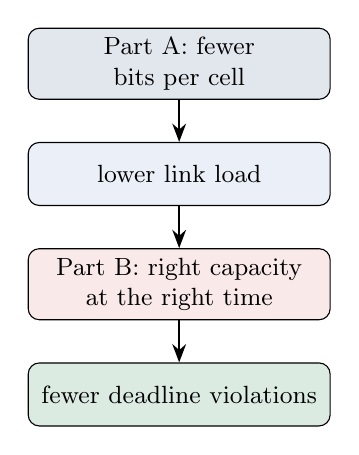
\begin{tikzpicture}[font=\small,>=Stealth,
  s/.style={draw,rounded corners,align=center,minimum height=0.8cm,text width=3.6cm}]
  \node[s,fill=iitblue!12] (a) at (0,0) {Part A: fewer bits per cell};
  \node[s,fill=soft] (l) at (0,-1.4) {lower link load};
  \node[s,fill=accent!10] (b) at (0,-2.8) {Part B: right capacity\\at the right time};
  \node[s,fill=good!15] (o) at (0,-4.2) {fewer deadline violations};
  \draw[->,thick] (a)--(l); \draw[->,thick] (l)--(b); \draw[->,thick] (b)--(o);
\end{tikzpicture}
\column{0.48\textwidth}
\begin{itemize}
  \item 9- to 6-bit mantissas lower the link load from 0.65 to 0.44.
  \item At load 0.65 the proposed rule \textbf{halves} the violations of reactive control: \textbf{1.96\,\% vs 3.90\,\%}.
  \item Part A keeps the link in the range where Part B is most effective.
\end{itemize}
\end{columns}
\end{frame}

% ------------------------------------------------------------------ 17
\begin{frame}{What builds on prior work and what is ours}
\footnotesize
\renewcommand{\arraystretch}{1.15}
\begin{tabular}{>{\raggedright\arraybackslash}p{2.4cm}>{\raggedright\arraybackslash}p{5.0cm}>{\raggedright\arraybackslash}p{6.6cm}}
\toprule
Area & Builds on & Our contribution \\
\midrule
IQ compression & O-RAN BFP, randomised SVD, delay sparsity & CSEE and RAS-BFP for real-time fronthaul, with bounds \\
Functional split & 3GPP split options, fixed at deployment & ACAFS: per-user split from the encoder's rank \\
Inversion & Newton--Schulz, Neumann, Marchenko--Pastur & RMT-WS: MP interval, Chebyshev start, warm start, certificate, Doppler law \\
DU kernel & LAPACK, AVX-512 & fused precoder kernel, 0.226 ms per slot \\
Allocation & newsvendor (Hadley--Whitin), point forecasts & deadline-feasible rate + per-cell KKT newsvendor for fronthaul \\
Strongest control & MaxWeight, policy search, used separately & BPN: one policy class containing both, beats both 10/10 \\
\bottomrule
\end{tabular}
\end{frame}

% ------------------------------------------------------------------ 18
\begin{frame}{Conclusion and future work}
\begin{columns}[T]
\column{0.55\textwidth}
\begin{block}{Conclusion}
\small
\begin{itemize}
  \item \textbf{Lighter fronthaul}: 13--16$\times$ compression (vs 4$\times$), 55--75\,\% split saving, 72\,\% with RU-side precoding.
  \item \textbf{Real-time DU}: whole precoder in 0.226~ms, 10--15$\times$ faster.
  \item \textbf{Smarter sharing}: KKT rule best of 12; BPN beats the strongest baselines in all 10 scenarios.
\end{itemize}
\end{block}
\column{0.42\textwidth}
\begin{block}{Future work}
\small
\begin{itemize}
  \item GPU / tensor-core kernels
  \item Real operator traces
  \item BPN as an RL xApp in the near-RT RIC
  \item Joint per-cell compression and allocation knob
  \item O-DU testbed deployment
\end{itemize}
\end{block}
\end{columns}
\vspace{0.3cm}
\centering\small B1 paper submitted to NCC 2027.
\end{frame}

% ------------------------------------------------------------------ 19
\begin{frame}
\centering
\vspace{1cm}
{\Huge \textcolor{iitblue}{Thank you}}\\[0.8cm]
{\Large Questions?}\\[1cm]
\small Harshvardhan Choudhary \quad Mayank Yadav\\
Guide: Dr. Sumit Gautam, Department of Electrical Engineering, IIT Indore
\end{frame}

\end{document}
